\subsubsection{Procedure}
Each participant was tested individually in a small meeting room (see Figure \ref{fig:test_setup}). Besides the participant, a facilitator and an observer was also present in the room. The test was split into seven parts:

\begin{enumerate}[noitemsep,nolistsep]
\item Consent form
\item Demographic and Introduction
\item Basic Navigation
\item Training
\item Tasks
\item Creative
\item Post-test Questionnaire
\end{enumerate} 

\subsubsection{Demographic and Introduction}
The participant were given a brief introduction and was subsequently presented with a consent form to allow video recording. The participants started by answering a demographic questionnaire on a laptop. After this they were introduced to a demo of the Camera Path Animator (see Section \ref{relatedWork}). They were told to move the player character by using WASD and then notice how the camera behaved accordingly. This was to give the participant context for the test and to introduce them to the concept of camera behaviour in an interactive environment. 

\begin{figure}[htbp]
\centering
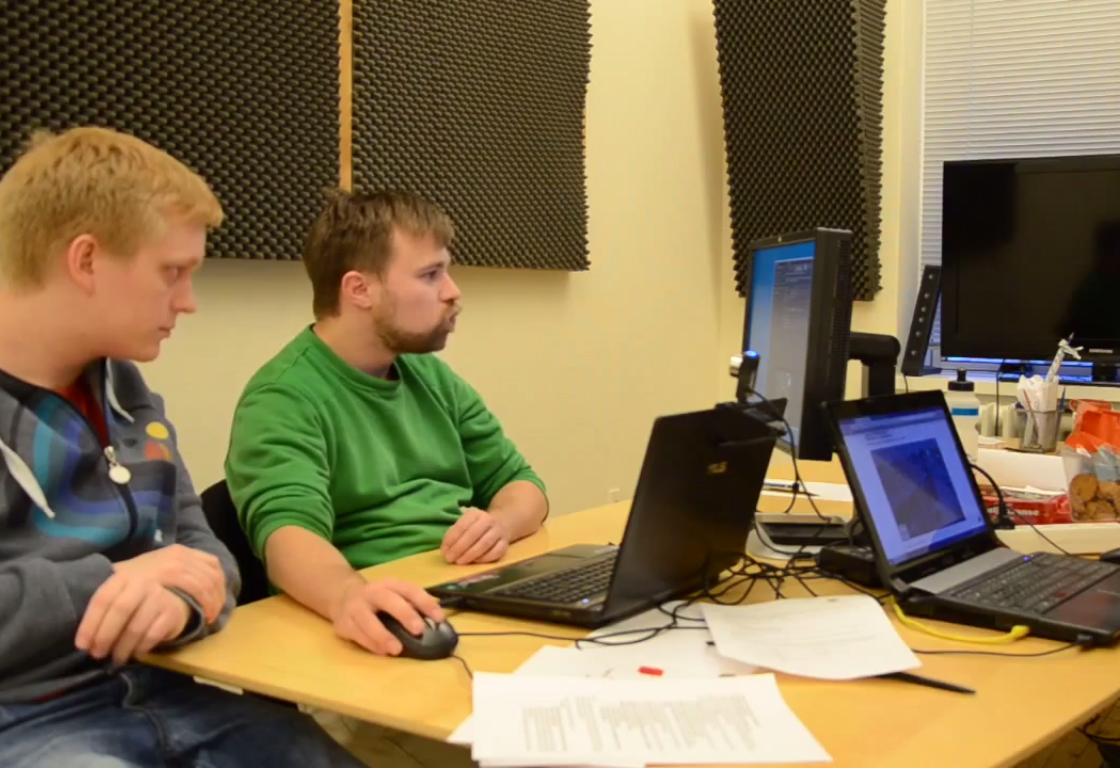
\includegraphics[width=0.3\textwidth]{Pics/test_setup}
\caption{The test participant used had two monitors at his disposal while working with the tool.}
\label{fig:framingConcept}
\end{figure}

\subsubsection{Basic Navigation}
The participants and facilitator sat down at another laptop with a second monitor connected. Here the facilitator gave the participant a basic introduction to Unity so that all participants had no problem understanding the Unity workspace layout, moving around with the scene view camera, changing the position and rotation of objects, etc. To ensure this, the participants was told to move the scene view camera to three positions in the scene (e.g. move camera above the green cube in Figure \ref{fig:sceneAll}). The participant was tasked to move the camera to three specific locations in the environment to ensure they felt comfortable in the workspace. 

\subsubsection{Training} 
After this the facilitator introduced the camera tool to the participant, first he explained the concept using a printed out version of Figure \ref{fig:framingConceptNew}, then he opened the tool in Unity and explained its features and functionalities. The participant tried each feature as they were introduced, e.g. when the facilitator explained how to place influence points and how to connect them, the participant was asked to try it for themselves. 

\subsubsection{Tasks}
When all features were explained, the participant was handed a piece of paper with five tasks. The tasks are as follows:

\begin{enumerate}[noitemsep,nolistsep]
\item Make the camera's field of view change.
\item Make the camera tilt upwards.
\item Make the camera look at the tall pink cylinder.
\item Make the camera go from a low perspective to bird’s-eye view.
\item Change the interpolation of one of the previous assignments by changing the animation curve.
\end{enumerate} 

The chosen tasks reflects five common features and tasks that's often used when setting up a framing and a camera interpolation. The participant had to solve the tasks themselves, the facilitator only intervened when the participant was struggling with something, asked a question, or at unforeseen occurrences (e.g. bugs). 

\subsubsection{Creative}
After this, the participant was introduced to a level with a modelled environment. They were then tasked to envision and sketch two ways for the camera to move as the play character moved through this environment, when they had two ideas, they were tasked to implement both of these using our camera tool. The facilitator remained as neutral as possible for this part of the test, but still intervened if they participant was struggling or encountered things like bugs.

\subsubsection{Post-test Questionnaire}
Finally, the participant went back to the first laptop and answered a post-test questionnaire. The participant was thanked and the test ended.